% Preliminaries: definitions and notation

\section{Preliminaries}\label{sec:preliminaries}

\subsection{Graph pebbling}

Let $G=(V,E)$ be a connected graph.
A \emph{pebble configuration} is a function $p\colon V\to\mathbb{Z}_{\ge 0}$.
A \emph{pebbling move} on an edge $\{u,v\}$ is allowed when $p(u)\ge 2$ and replaces
$p$ by $p'$ with $p'(u)=p(u)-2$, $p'(v)=p(v)+1$, and $p'(w)=p(w)$ for $w\notin\{u,v\}$.
We say that a configuration $p$ can \emph{pebble} (or \emph{reach}) a target vertex $t$
if some finite sequence of pebbling moves produces a configuration with at least one pebble on~$t$.

For a fixed target $t$, the \emph{$t$-pebbling number} is
\[
\pi(G,t)=\min\{S\in\mathbb{Z}_{>0} : \text{every configuration with exactly $S$ pebbles can pebble $t$}\}.
\]
The \emph{pebbling number} of $G$ is
\[
\pi(G)=\max_{t\in V}\pi(G,t).
\]

\begin{lemma}[Monotonicity {\cite[Prop.~2]{Bunde2008}}]\label{lem:mono}
Fix a target~$t$. If $k\ge \pi(G,t)$, then every configuration with exactly $k$
pebbles can pebble~$t$.
\end{lemma}

\begin{proof}
See~\cite{Bunde2008,Hurlbert1999}.
\end{proof}

\subsection{Double-tailed tadpole graphs}\label{sec:tadpole-def}

\begin{definition}[Double-tailed tadpole graph $T(3,s_1,s_2)$]
Fix integers $s_1,s_2\ge 1$.
The graph $T(3,s_1,s_2)$ consists of:
\begin{itemize}
  \item a triangle on vertices $\{a,b,c\}$;
  \item a path of length $s_1$ joining $a$ to a leaf $u_L$;
  \item a path of length $s_2$ joining $b$ to a leaf $u_R$;
  \item no edges from $c$ to either tail.
\end{itemize}
The graph has $n=3+s_1+s_2$ vertices and diameter
\[
d=s_1+s_2+1=\operatorname{diam}(T(3,s_1,s_2)).
\]
\end{definition}

\begin{figure}[ht]
\centering
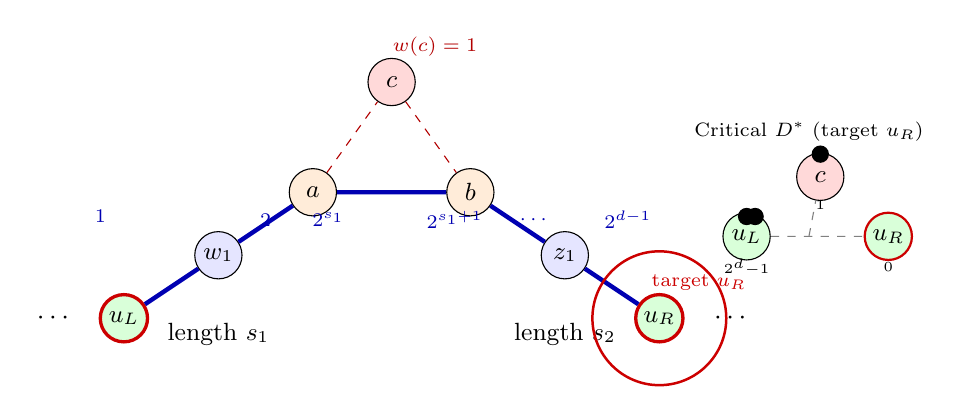
\begin{tikzpicture}[
  vtx/.style={circle, draw, minimum size=6mm, inner sep=0pt, font=\small},
  tail/.style={vtx, fill=blue!10},
  tri/.style={vtx, fill=orange!15},
  apex/.style={vtx, fill=red!15},
  leaf/.style={vtx, fill=green!15},
  target/.style={leaf, draw=red!80!black, line width=1.2pt},
  spine/.style={line width=1.6pt, draw=blue!70!black},
  branch/.style={dashed, draw=red!70!black},
  peb/.style={circle, fill=black, inner sep=0pt, minimum size=2.2mm}
]
  \node[tri] (a) at (0,0) {$a$};
  \node[tri] (b) at (2,0) {$b$};
  \node[apex] (c) at (1,1.4) {$c$};
  \draw (a)--(b);
  \draw[branch] (a)--(c)--(b);
  \node[tail] (w1) at (-1.2,-0.8) {$w_1$};
  \node[target] (uL) at (-2.4,-1.6) {$u_L$};
  \draw[spine] (uL)--(w1)--(a)--(b);
  \node at (-3.3,-1.6) {$\cdots$};
  \node at (-1.2,-1.8) {\small length $s_1$};
  \node[tail] (z1) at (3.2,-0.8) {$z_1$};
  \node[target] (uR) at (4.4,-1.6) {$u_R$};
  \draw[spine] (b)--(z1)--(uR);
  \node at (5.3,-1.6) {$\cdots$};
  \node at (3.2,-1.8) {\small length $s_2$};
  \node[font=\scriptsize, blue!70!black] at (-2.7,-0.3) {$1$};
  \node[font=\scriptsize, blue!70!black] at (-0.6,-0.35) {$2$};
  \node[font=\scriptsize, blue!70!black] at (0.2,-0.35) {$2^{s_1}$};
  \node[font=\scriptsize, blue!70!black] at (1.8,-0.35) {$2^{s_1+1}$};
  \node[font=\scriptsize, blue!70!black] at (2.8,-0.35) {$\cdots$};
  \node[font=\scriptsize, blue!70!black] at (4.0,-0.35) {$2^{d-1}$};
  \node[font=\scriptsize, red!70!black] at (1.55,1.85) {$w(c)=1$};
  \node[font=\scriptsize, red!80!black] at (4.9,-1.15) {target $u_R$};
  \draw[red!80!black, line width=0.9pt] (4.4,-1.6) circle (8.5mm);

  \begin{scope}[shift={(6.3,-0.2)}, scale=0.72]
    \node[font=\scriptsize] at (0,1.35) {Critical $D^*$ (target $u_R$)};
    \node[vtx, fill=green!15] (duL) at (-1.1,-0.5) {$u_L$};
    \node[vtx, fill=red!15] (dc) at (0.2,0.55) {$c$};
    \node[vtx, fill=green!15, draw=red!80!black, line width=0.8pt] (duR) at (1.4,-0.5) {$u_R$};
    \draw[dashed, gray] (duL)--(0,-0.5)--(duR);
    \draw[dashed, gray] (0,-0.5)--(dc);
    \node[font=\tiny] at (-1.1,-1.05) {$2^d{-}1$};
    \node[font=\tiny] at (0.2,0.05) {$1$};
    \node[font=\tiny] at (1.4,-1.05) {$0$};
    \node[peb] at (-1.1,-0.15) {};
    \node[peb] at (-0.95,-0.15) {};
    \node[peb] at (0.2,0.95) {};
  \end{scope}
\end{tikzpicture}
\caption{$T(3,s_1,s_2)$ and the objects used later.
The bold spine is the Hamiltonian path $u_L\to\cdots\to u_R$ of
Section~\ref{sec:path-spine-wf}; dashed edges mark the branch at~$c$.
Blue labels are path-spine weights toward target~$u_R$ (red circle).
The inset shows the critical configuration~$D^*$ (Definition~\ref{def:critical}).}
\label{fig:tadpole-schematic}
\end{figure}

\subsection{Critical configuration}\label{sec:critical-def}

\begin{definition}[Critical configuration $D^*$]\label{def:critical}
Fix target $u_R$ and let $d=s_1+s_2+1$.
Define the configuration $D^*$ by
\[
D^*(u_L)=2^d-1,\qquad D^*(c)=1,\qquad D^*(v)=0 \text{ for all other vertices } v.
\]
Then $|D^*| = 2^d$.
\end{definition}

At $S=2^d$, every instance in Table~\ref{tab:critical} fails in a configuration
matching~$D^*$ up to automorphism.
That $D^*$ cannot pebble~$u_R$ is proved in Section~\ref{sec:lower-bound}; the value
$\pi(G)=2^d+1$ is Theorem~\ref{thm:exact}.
